\documentclass[14pt]{extbook}
\usepackage{multicol, enumerate, enumitem, hyperref, color, soul, setspace, parskip, fancyhdr} %General Packages
\usepackage{amssymb, amsthm, amsmath, bbm, latexsym, units, mathtools} %Math Packages
\everymath{\displaystyle} %All math in Display Style
% Packages with additional options
\usepackage[headsep=0.5cm,headheight=12pt, left=1 in,right= 1 in,top= 1 in,bottom= 1 in]{geometry}
\usepackage[usenames,dvipsnames]{xcolor}
\usepackage{dashrule}  % Package to use the command below to create lines between items
\newcommand{\litem}[1]{\item#1\hspace*{-1cm}\rule{\textwidth}{0.4pt}}
\pagestyle{fancy}
\lhead{Makeup Progress Quiz -1}
\chead{}
\rhead{Version B}
\lfoot{7547-2949}
\cfoot{}
\rfoot{Fall 2020}
\begin{document}

\begin{enumerate}
\litem{
Describe the end behavior of the polynomial below.\[ f(x) = -9(x + 4)^{3}(x - 4)^{6}(x + 5)^{2}(x - 5)^{3} \]\begin{enumerate}[label=\Alph*.]
\begin{multicols}{2}\item 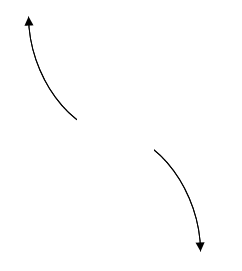
\includegraphics[width = 0.3\textwidth]{../Figures/polyEndBehaviorAB.png}\item 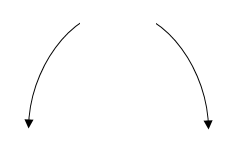
\includegraphics[width = 0.3\textwidth]{../Figures/polyEndBehaviorBB.png}\item 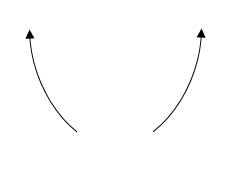
\includegraphics[width = 0.3\textwidth]{../Figures/polyEndBehaviorCB.png}\item 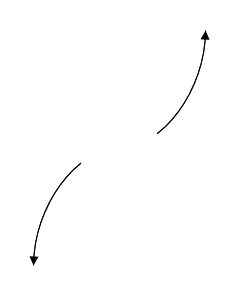
\includegraphics[width = 0.3\textwidth]{../Figures/polyEndBehaviorDB.png}\end{multicols}\item None of the above.
\end{enumerate} }
\litem{
Describe the zero behavior of the zero $x = 2$ of the polynomial below.\[ f(x) = 9(x + 4)^{6}(x - 4)^{4}(x - 2)^{9}(x + 2)^{6} \]\begin{enumerate}[label=\Alph*.]
\begin{multicols}{2}\item 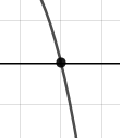
\includegraphics[width = 0.3\textwidth]{../Figures/polyZeroBehaviorCopyAB.png}\item 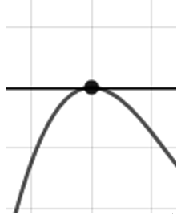
\includegraphics[width = 0.3\textwidth]{../Figures/polyZeroBehaviorCopyBB.png}\item 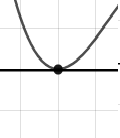
\includegraphics[width = 0.3\textwidth]{../Figures/polyZeroBehaviorCopyCB.png}\item 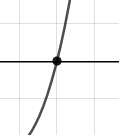
\includegraphics[width = 0.3\textwidth]{../Figures/polyZeroBehaviorCopyDB.png}\end{multicols}\item None of the above.
\end{enumerate} }
\litem{
Construct the lowest-degree polynomial given the zeros below. Then, choose the intervals that contain the coefficients of the polynomial in the form $x^3+bx^2+cx+d$.\[ -5 - 4 i \text{ and } 2 \]\begin{enumerate}[label=\Alph*.]
\item \( b \in [7, 11], c \in [16.6, 24.7], \text{ and } d \in [-82.5, -81] \)
\item \( b \in [0, 5], c \in [1.6, 2.3], \text{ and } d \in [-9.2, -7.7] \)
\item \( b \in [0, 5], c \in [2.8, 4.4], \text{ and } d \in [-11.9, -8.9] \)
\item \( b \in [-10, -4], c \in [16.6, 24.7], \text{ and } d \in [78.5, 82.4] \)
\item \( \text{None of the above.} \)

\end{enumerate} }
\litem{
Describe the zero behavior of the zero $x = -6$ of the polynomial below.\[ f(x) = -7(x + 6)^{8}(x - 6)^{9}(x - 3)^{6}(x + 3)^{9} \]\begin{enumerate}[label=\Alph*.]
\begin{multicols}{2}\item 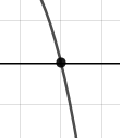
\includegraphics[width = 0.3\textwidth]{../Figures/polyZeroBehaviorAB.png}\item 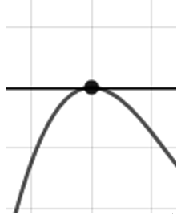
\includegraphics[width = 0.3\textwidth]{../Figures/polyZeroBehaviorBB.png}\item 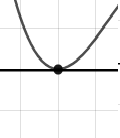
\includegraphics[width = 0.3\textwidth]{../Figures/polyZeroBehaviorCB.png}\item 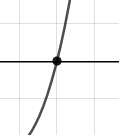
\includegraphics[width = 0.3\textwidth]{../Figures/polyZeroBehaviorDB.png}\end{multicols}\item None of the above.
\end{enumerate} }
\litem{
Which of the following equations \textit{could} be of the graph presented below?
\begin{center}
    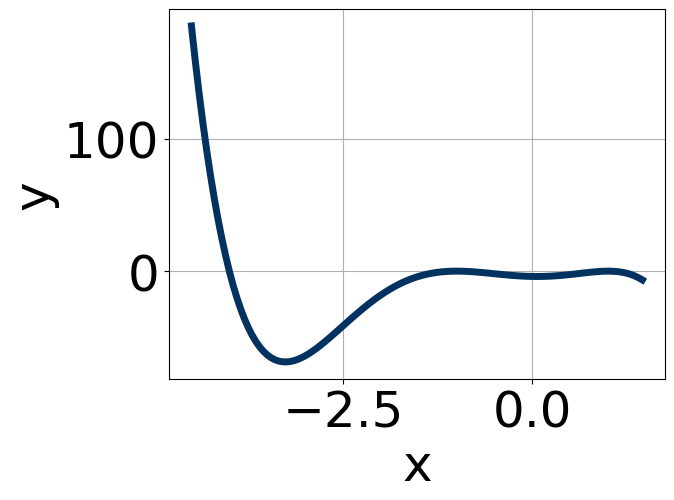
\includegraphics[width=0.5\textwidth]{../Figures/polyGraphToFunctionCopyB.png}
\end{center}
\begin{enumerate}[label=\Alph*.]
\item \( 6(x + 1)^{10} (x - 1)^{6} (x + 4)^{6} \)
\item \( -6(x + 1)^{4} (x - 1)^{5} (x + 4)^{8} \)
\item \( -9(x + 1)^{10} (x - 1)^{9} (x + 4)^{11} \)
\item \( -7(x + 1)^{6} (x - 1)^{6} (x + 4)^{9} \)
\item \( 15(x + 1)^{8} (x - 1)^{4} (x + 4)^{5} \)

\end{enumerate} }
\litem{
Which of the following equations \textit{could} be of the graph presented below?
\begin{center}
    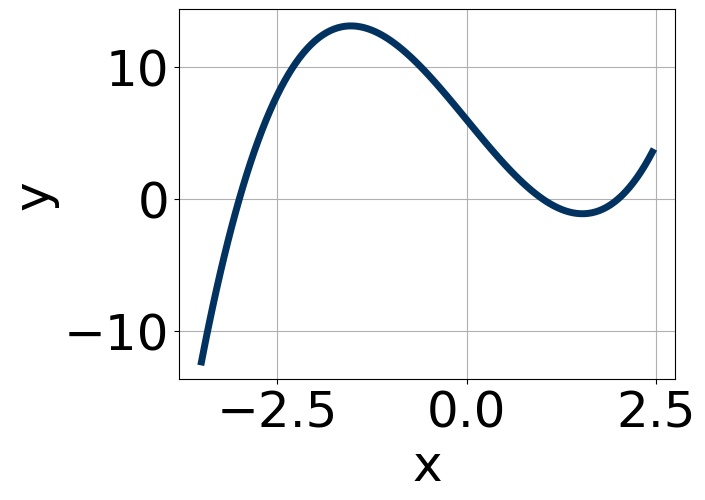
\includegraphics[width=0.5\textwidth]{../Figures/polyGraphToFunctionB.png}
\end{center}
\begin{enumerate}[label=\Alph*.]
\item \( -3(x - 2)^{9} (x + 3)^{11} (x - 1)^{9} \)
\item \( 17(x - 2)^{10} (x + 3)^{7} (x - 1)^{7} \)
\item \( -18(x - 2)^{8} (x + 3)^{9} (x - 1)^{5} \)
\item \( 20(x - 2)^{4} (x + 3)^{10} (x - 1)^{9} \)
\item \( 6(x - 2)^{9} (x + 3)^{9} (x - 1)^{7} \)

\end{enumerate} }
\litem{
Describe the end behavior of the polynomial below.\[ f(x) = 3(x - 4)^{4}(x + 4)^{5}(x + 3)^{5}(x - 3)^{6} \]\begin{enumerate}[label=\Alph*.]
\begin{multicols}{2}\item 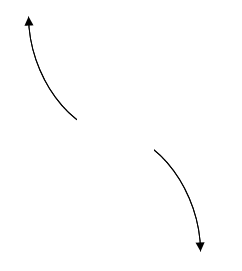
\includegraphics[width = 0.3\textwidth]{../Figures/polyEndBehaviorCopyAB.png}\item 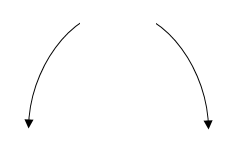
\includegraphics[width = 0.3\textwidth]{../Figures/polyEndBehaviorCopyBB.png}\item 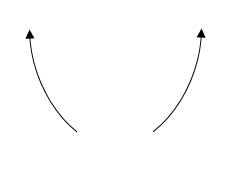
\includegraphics[width = 0.3\textwidth]{../Figures/polyEndBehaviorCopyCB.png}\item 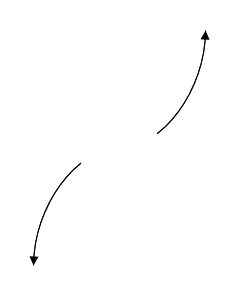
\includegraphics[width = 0.3\textwidth]{../Figures/polyEndBehaviorCopyDB.png}\end{multicols}\item None of the above.
\end{enumerate} }
\litem{
Construct the lowest-degree polynomial given the zeros below. Then, choose the intervals that contain the coefficients of the polynomial in the form $ax^3+bx^2+cx+d$.\[ \frac{6}{5}, \frac{4}{5}, \text{ and } \frac{-5}{2} \]\begin{enumerate}[label=\Alph*.]
\item \( a \in [50, 56], b \in [225, 228], c \in [298, 302], \text{ and } d \in [113, 124] \)
\item \( a \in [50, 56], b \in [15, 26], c \in [-203, -196], \text{ and } d \in [113, 124] \)
\item \( a \in [50, 56], b \in [140, 148], c \in [0, 13], \text{ and } d \in [-125, -119] \)
\item \( a \in [50, 56], b \in [15, 26], c \in [-203, -196], \text{ and } d \in [-125, -119] \)
\item \( a \in [50, 56], b \in [-26, -18], c \in [-203, -196], \text{ and } d \in [-125, -119] \)

\end{enumerate} }
\litem{
Construct the lowest-degree polynomial given the zeros below. Then, choose the intervals that contain the coefficients of the polynomial in the form $x^3+bx^2+cx+d$.\[ -5 + 5 i \text{ and } -1 \]\begin{enumerate}[label=\Alph*.]
\item \( b \in [-12, -5], c \in [60, 64], \text{ and } d \in [-51, -40] \)
\item \( b \in [7, 18], c \in [60, 64], \text{ and } d \in [48, 53] \)
\item \( b \in [-3, 9], c \in [0, 11], \text{ and } d \in [2, 15] \)
\item \( b \in [-3, 9], c \in [-6, -2], \text{ and } d \in [-5, -2] \)
\item \( \text{None of the above.} \)

\end{enumerate} }
\litem{
Construct the lowest-degree polynomial given the zeros below. Then, choose the intervals that contain the coefficients of the polynomial in the form $ax^3+bx^2+cx+d$.\[ \frac{-6}{5}, \frac{-1}{2}, \text{ and } \frac{4}{5} \]\begin{enumerate}[label=\Alph*.]
\item \( a \in [40, 53], b \in [43, 50], c \in [-38, -36], \text{ and } d \in [20, 26] \)
\item \( a \in [40, 53], b \in [-133, -118], c \in [93, 99], \text{ and } d \in [-28, -21] \)
\item \( a \in [40, 53], b \in [-78, -71], c \in [-6, 0], \text{ and } d \in [20, 26] \)
\item \( a \in [40, 53], b \in [-54, -41], c \in [-38, -36], \text{ and } d \in [20, 26] \)
\item \( a \in [40, 53], b \in [43, 50], c \in [-38, -36], \text{ and } d \in [-28, -21] \)

\end{enumerate} }
\end{enumerate}

\end{document}